
\clearpage
\textcolor{blue}{EQ Comments: Histogram for all login days, not only those used in our main analysis}

\begin{figure}[hbt!]
	\centering%
	\caption{Histogram of Stock Prices}%
	\label{fig:histogram_prices}%
	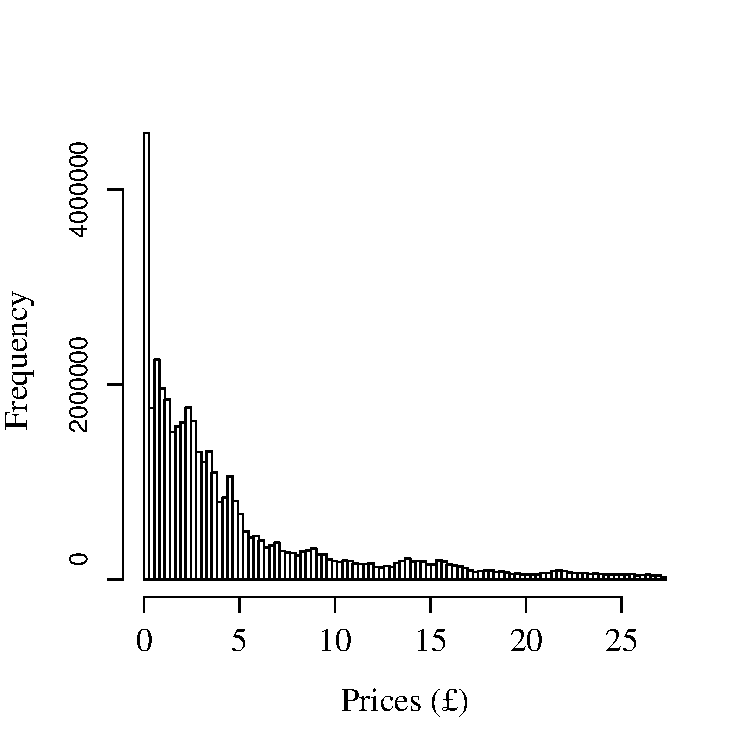
\includegraphics[width=.6\textwidth]{figures/prices_hist_login_days.pdf}
	\fignote{Figure shows the histogram of prices on login days. Outliers above the 95 percentile are excluded.}
\end{figure}



\clearpage
\textcolor{blue}{EQ Comments: Patterns are unobservable if using all login days without any restriction}

\begin{figure}[hbt!]
	\caption{Leftmost Stock Price Digit and Probability of Sale \\ All Login Days}%
	\label{fig:left_digit_sell_increase}%
	\centering%	

		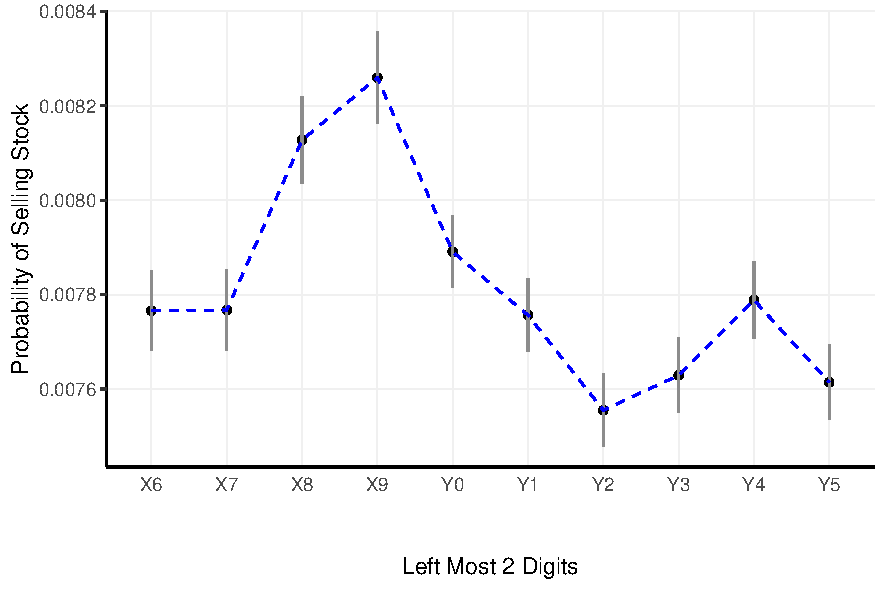
\includegraphics[width=0.6\textwidth]{figures/Left2all_data_probCI.pdf}

	\fignote{£$Y$ in the X-axes is equivalent to £$X+1$ (e.g., £X9 could include £0.19, £1.9, £19, etc., while £Y0 could include £0.20, £2.0, £20, etc.). }
\end{figure}


\clearpage
\textcolor{blue}{EQ: Robustness 1: Same patterns in sub-samples of equal bin size for our main sample (quarterly sample and login days)}

\begin{figure}[hbt!]
	\caption{Leftmost Stock Price Digit and Probability of Sale \\ Prices Increasing Sample by Price Range}%
	\label{fig:left_digit_sell_increase}%
	\centering%	
	\bigskip
	\subfigure[Price = \pounds0.11 to \pounds1.01]{
		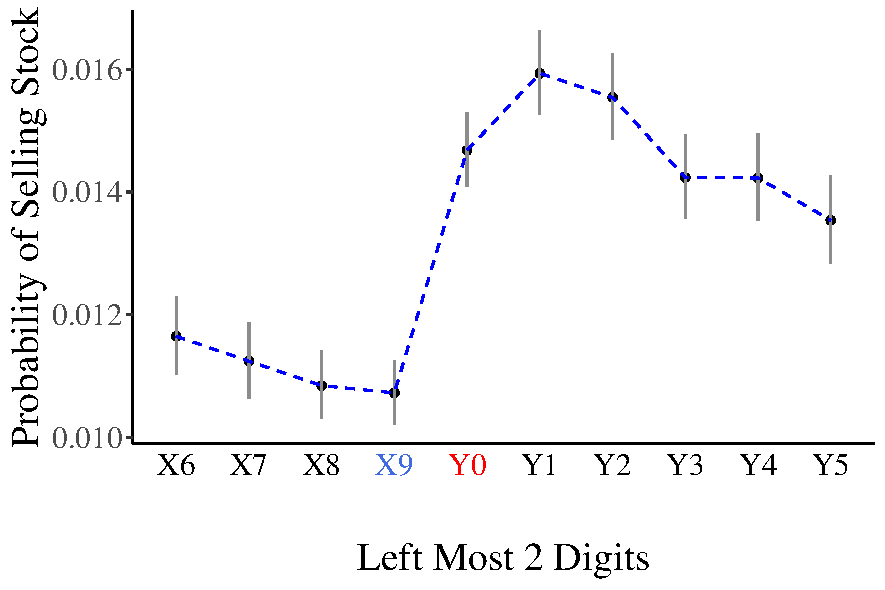
\includegraphics[width=0.45\textwidth]{figures/Left2increases_1pbin_CI_quarter.pdf}
		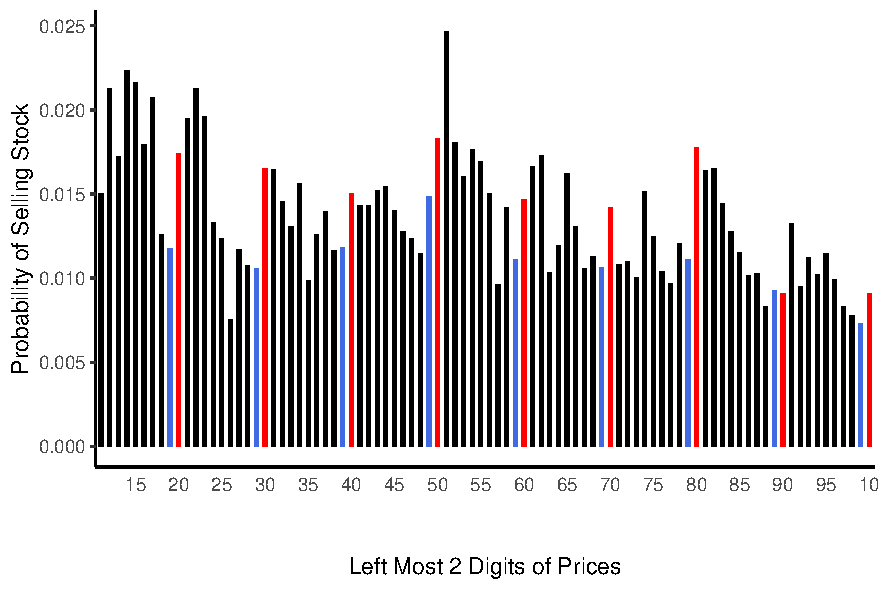
\includegraphics[width=0.45\textwidth]{figures/2left_increase_bin1p_quarter.pdf}
	}
	\subfigure[Price = \pounds1.01 to \pounds10.1]{
		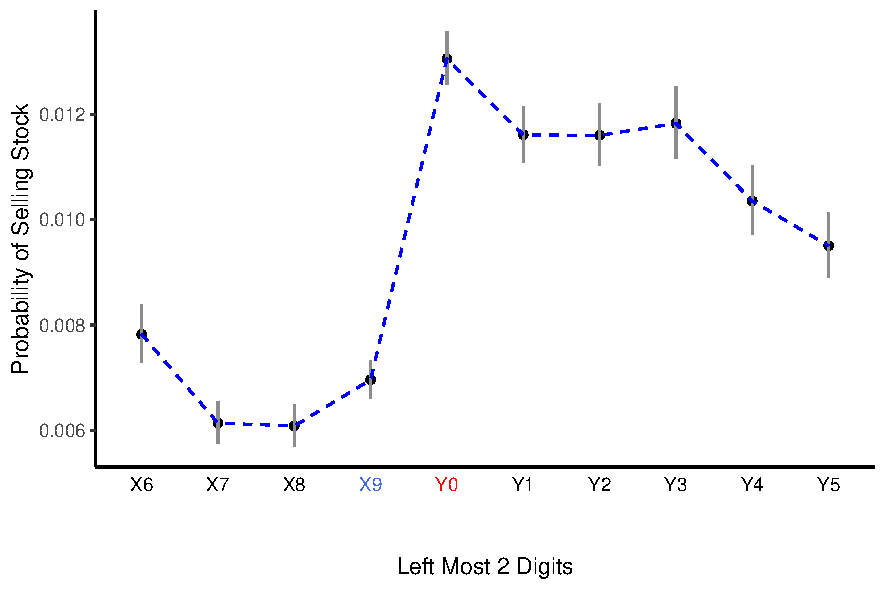
\includegraphics[width=0.45\textwidth]{figures/Left2increases_10pbin_CI_quarter.pdf}
		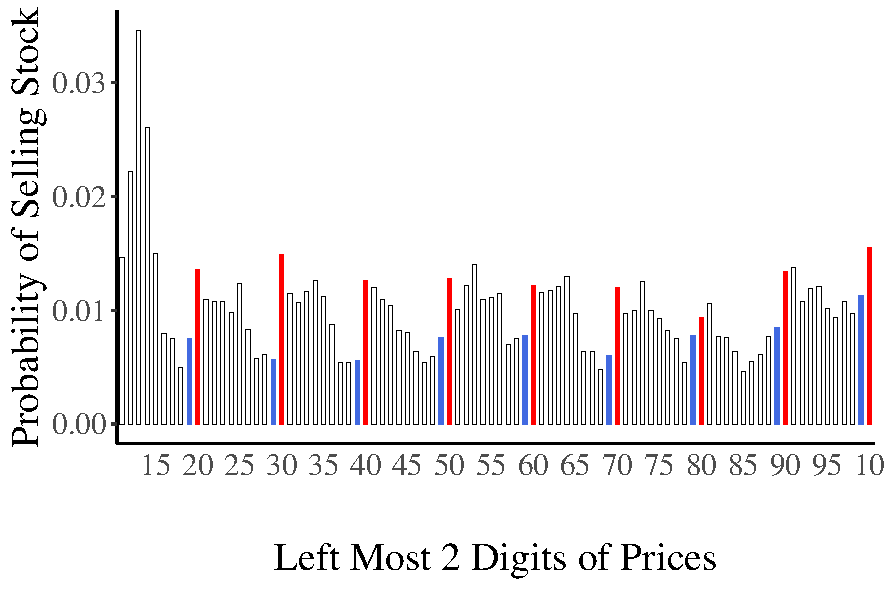
\includegraphics[width=0.45\textwidth]{figures/2left_increase_bin10p_quarter.pdf}
	}
	\subfigure[Price = \pounds11 to \pounds101]{
		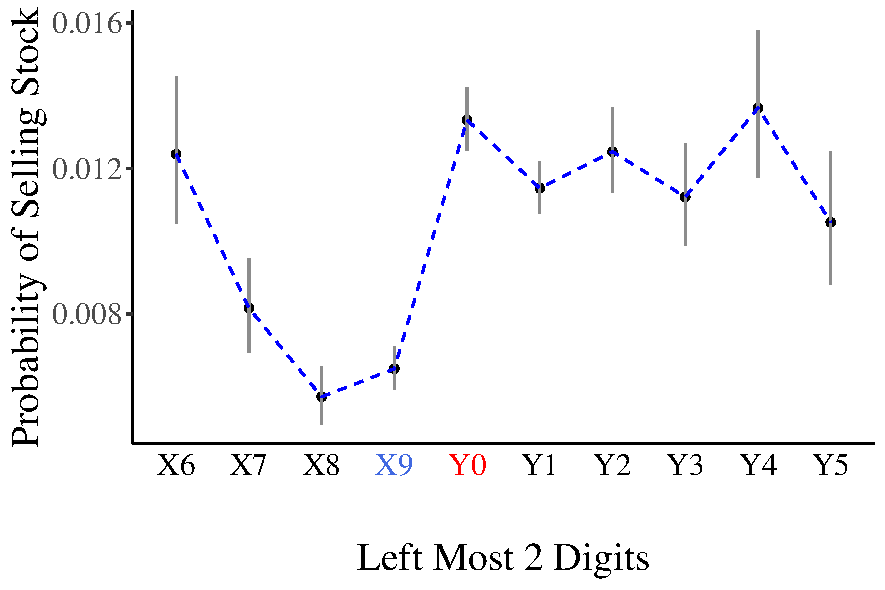
\includegraphics[width=0.45\textwidth]{figures/Left2increases_1poundbin_CI_quarter.pdf}
		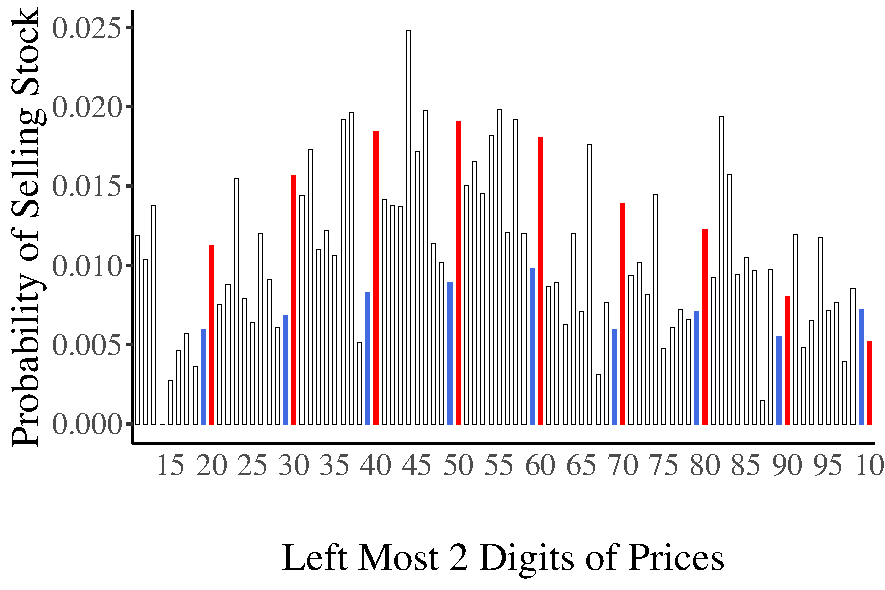
\includegraphics[width=0.45\textwidth]{figures/2left_increase_bin1pound_quarter.pdf}
	}
	\fignote{£$Y$ in the X-axes is equivalent to £$X+1$ (e.g., £X9 could include £0.19, £1.9, £19, etc., while £Y0 could include £0.20, £2.0, £20, etc.). Panels A, B and C show equal size bins of 1p, 10p and £1, respectively. Panel A corresponds to 25\% of the observations in the prices increasing sample; Panel B, to 55\%; and Panel C, to 8\%.}
\end{figure}

\begin{figure}[hbt!]
	\caption{Leftmost Stock Price Digit and Probability of Sale \\ Prices Decreasing Sample by Price Range}%
	\label{fig:left_digit_sell_decrease}%
	\centering%	
	\bigskip
	\subfigure[Price = \pounds0.10 to \pounds1.00]{
		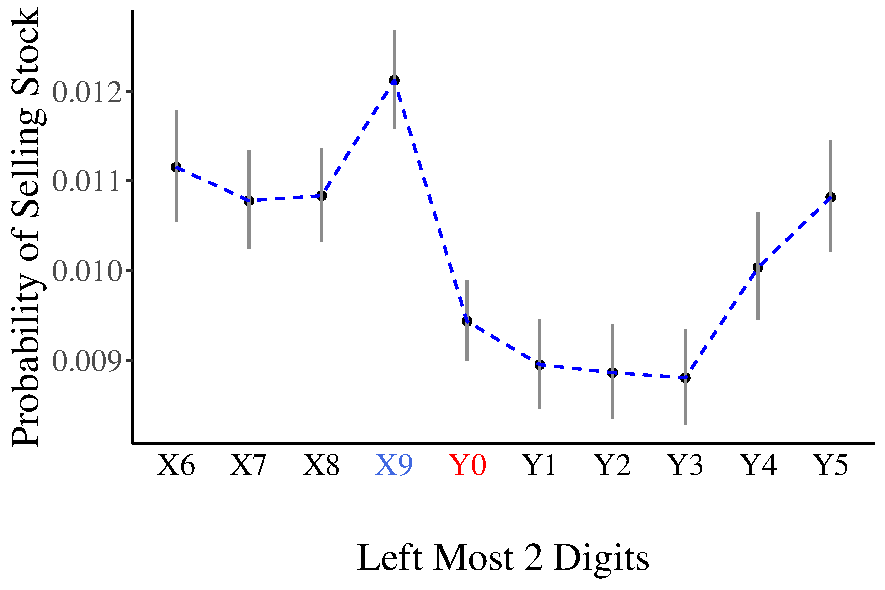
\includegraphics[width=0.45\textwidth]{figures/Left2decreases_1pbin_CI_quarter.pdf}
		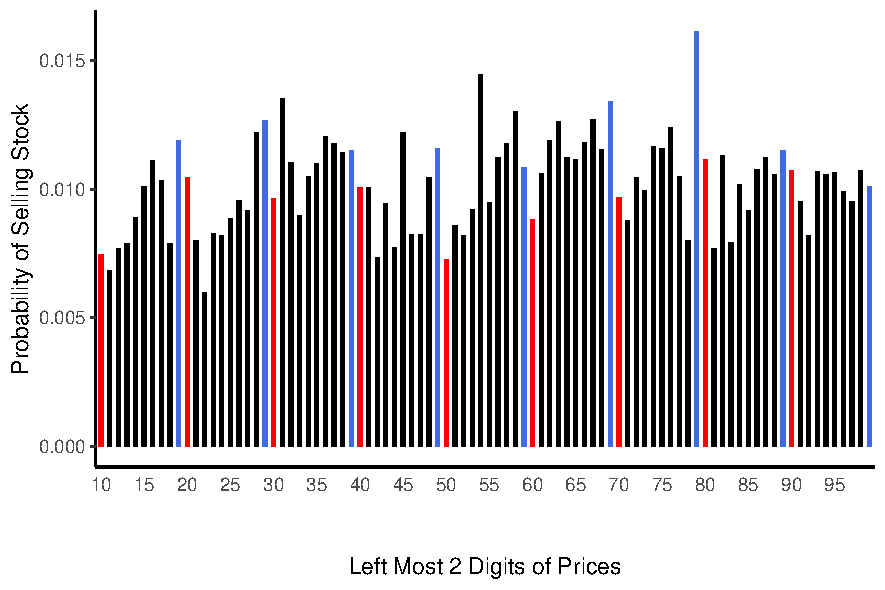
\includegraphics[width=0.45\textwidth]{figures/2left_decrease_bin1p_quarter.pdf}
	}
	\subfigure[Price = \pounds1.00 to \pounds10.0]{
		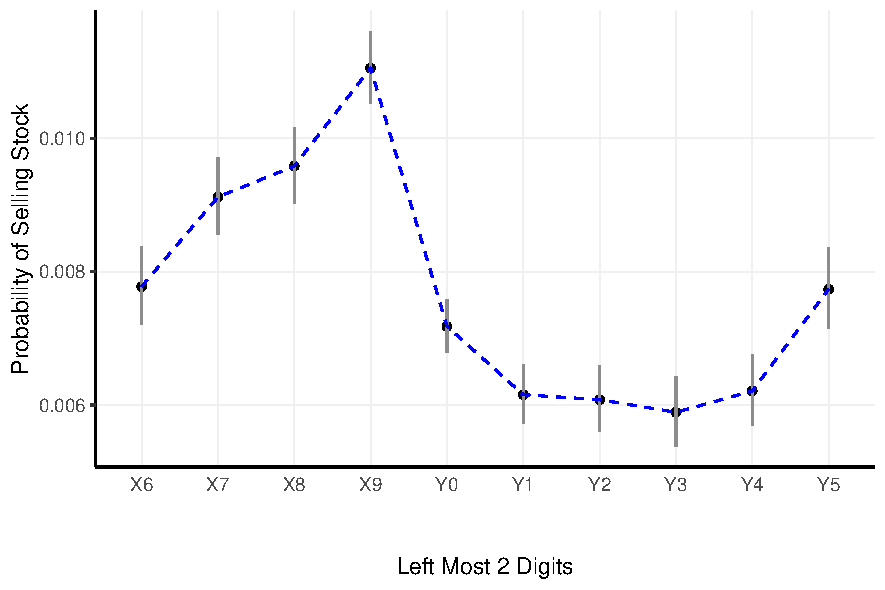
\includegraphics[width=0.45\textwidth]{figures/Left2decreases_10pbin_CI_quarter.pdf}
		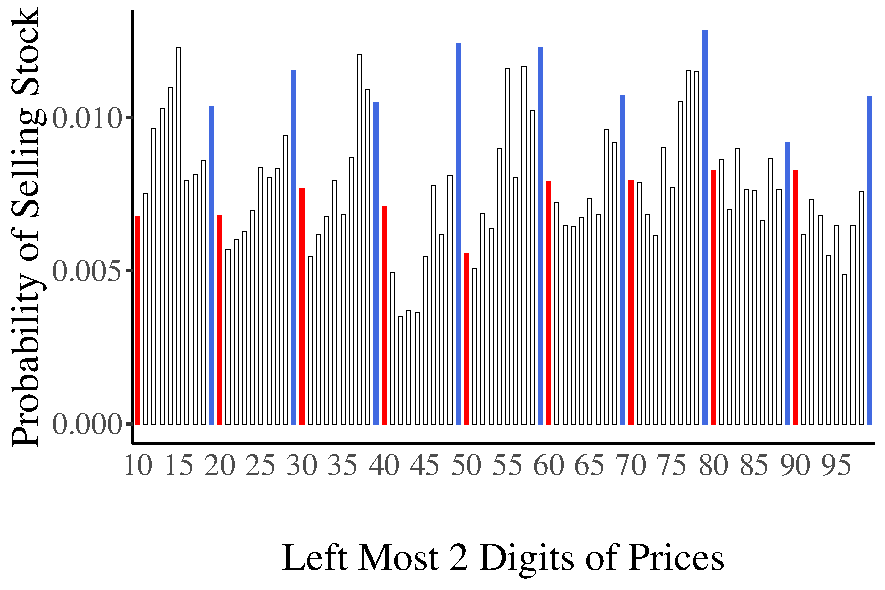
\includegraphics[width=0.45\textwidth]{figures/2left_decrease_bin10p_quarter.pdf}
	}
	\subfigure[Price = \pounds10 to \pounds100]{
		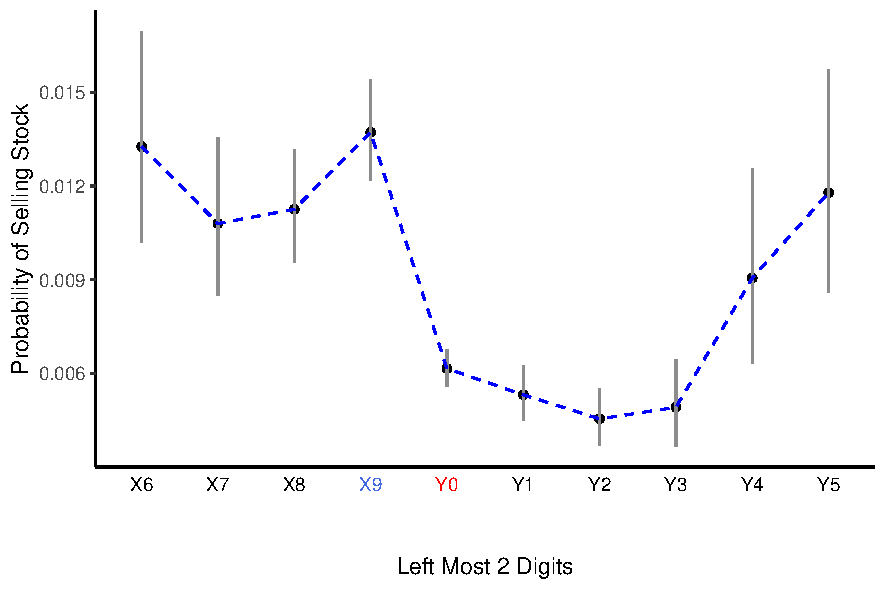
\includegraphics[width=0.45\textwidth]{figures/Left2decreases_1poundbin_CI_quarter.pdf}
		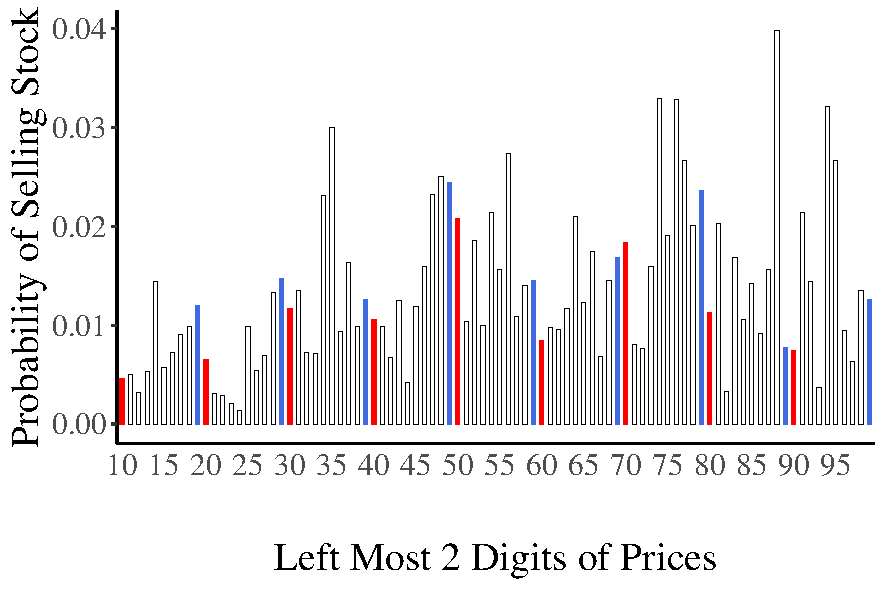
\includegraphics[width=0.45\textwidth]{figures/2left_decrease_bin1pound_quarter.pdf}
	}
	\fignote{£$Y$ in the X-axes is equivalent to £$X+1$ (e.g., £X9 could include £0.19, £1.9, £19, etc., while £Y0 could include £0.20, £2.0, £20, etc.). Panels A, B and C show equal size bins of 1p, 10p and £1, respectively. Panel A corresponds to 27\% of the observations in the prices decreasing sample; Panel B, to 43\%; and Panel C, to 7\%.}
\end{figure}


\clearpage
\textcolor{blue}{EQ: Robustness 2: Same patterns in monthly and annual samples (login days)}

\begin{figure}[hbt!]
	\caption{Leftmost Stock Price Digit and Probability of Sale, Monthly Sample}%
	\label{fig:left_digit_sell}%
	\centering%	
	\bigskip
	\subfigure[Price Increasing]{
		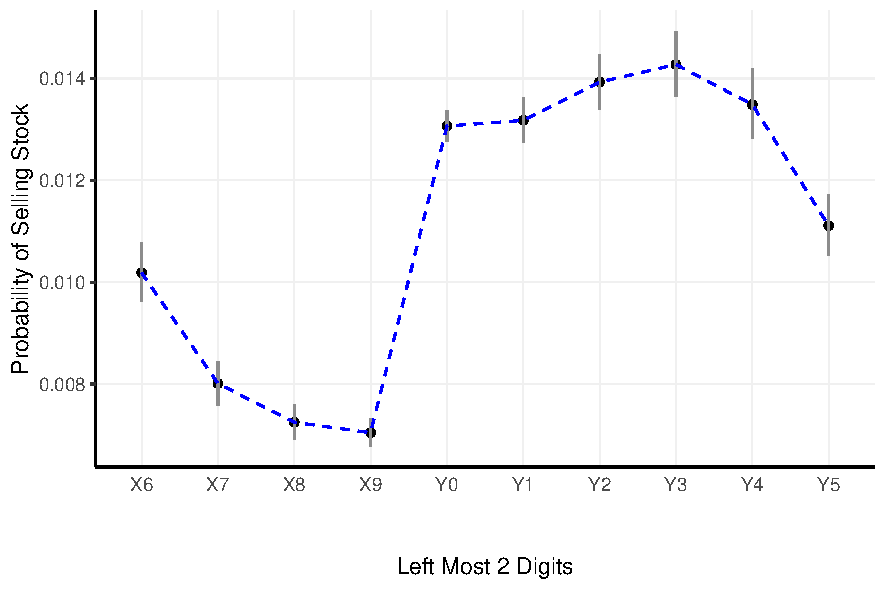
\includegraphics[width=0.45\textwidth]{figures/Left2increase_probCI_month.pdf}
		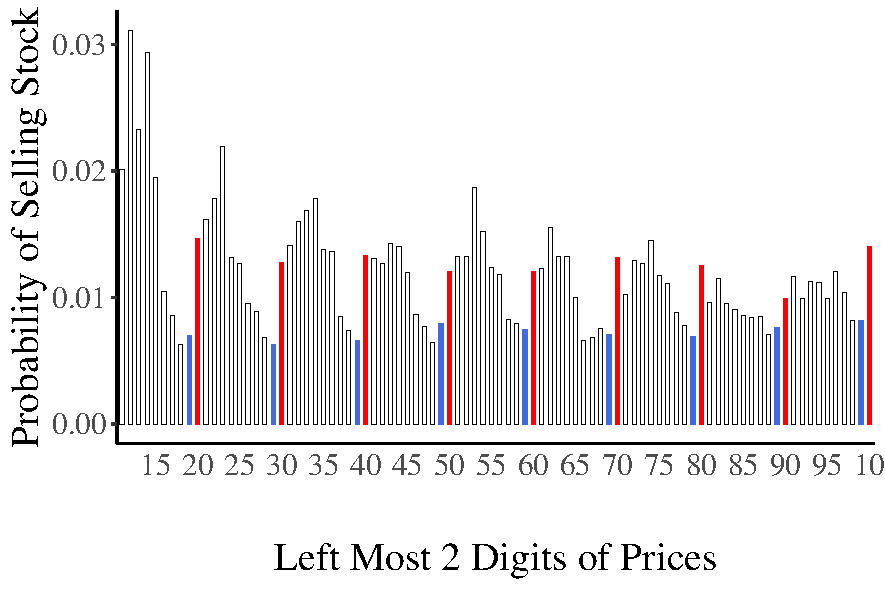
\includegraphics[width=0.45\textwidth]{figures/2left_increase_month.pdf}	
	}
	\subfigure[Price Decreasing]{
		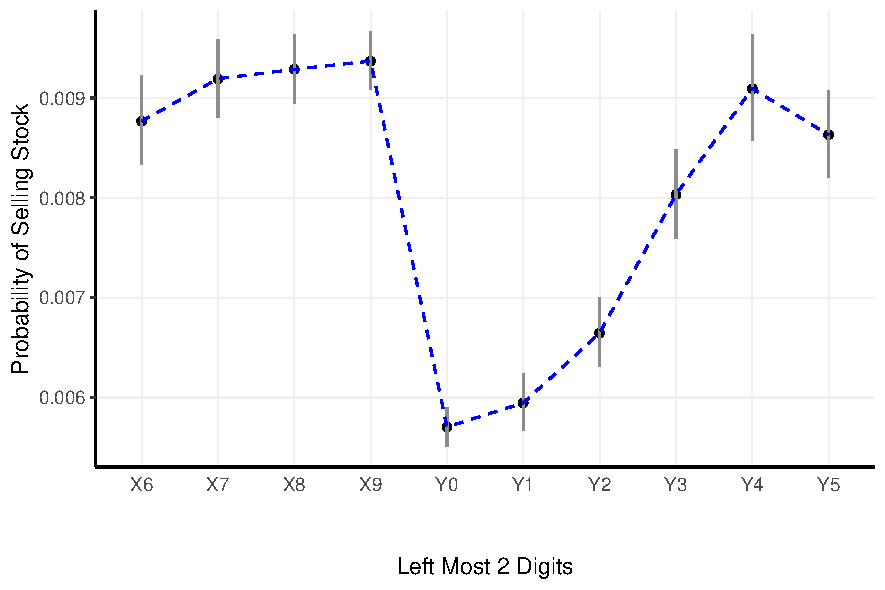
\includegraphics[width=0.45\textwidth]{figures/Left2decrease_probCI_month.pdf}
		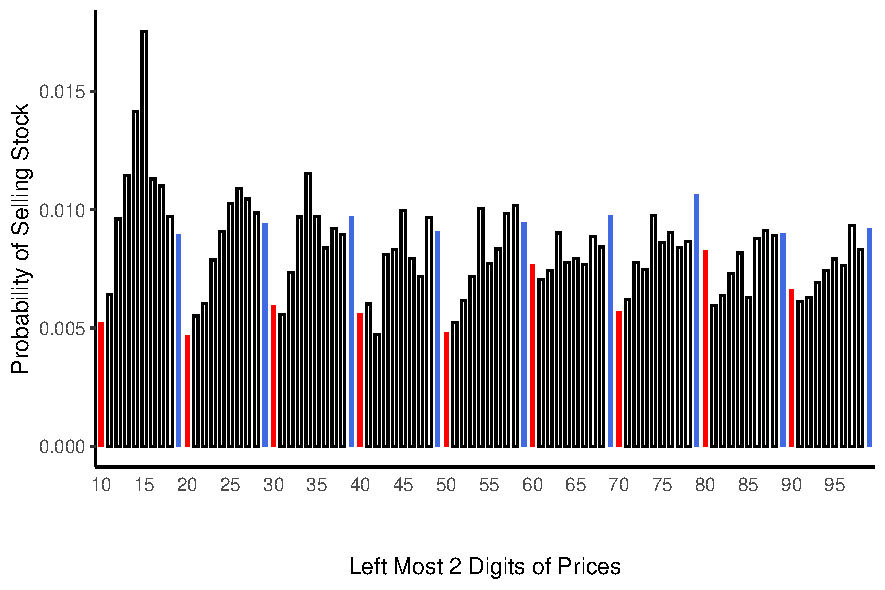
\includegraphics[width=0.45\textwidth]{figures/2left_decrease_month.pdf}	
	}
	\fignote{£$Y$ in the X-axes is equivalent to £$X+1$ (e.g., £X9 could include £0.19, £1.9, £19, etc., while £Y0 could include £0.20, £2.0, £20, etc.).}
\end{figure}

\begin{figure}[hbt!]
	\caption{Leftmost Stock Price Digit and Probability of Sale, Annual Sample}%
	\label{fig:left_digit_sell}%
	\centering%	
	\bigskip
	\subfigure[Price Increasing]{
		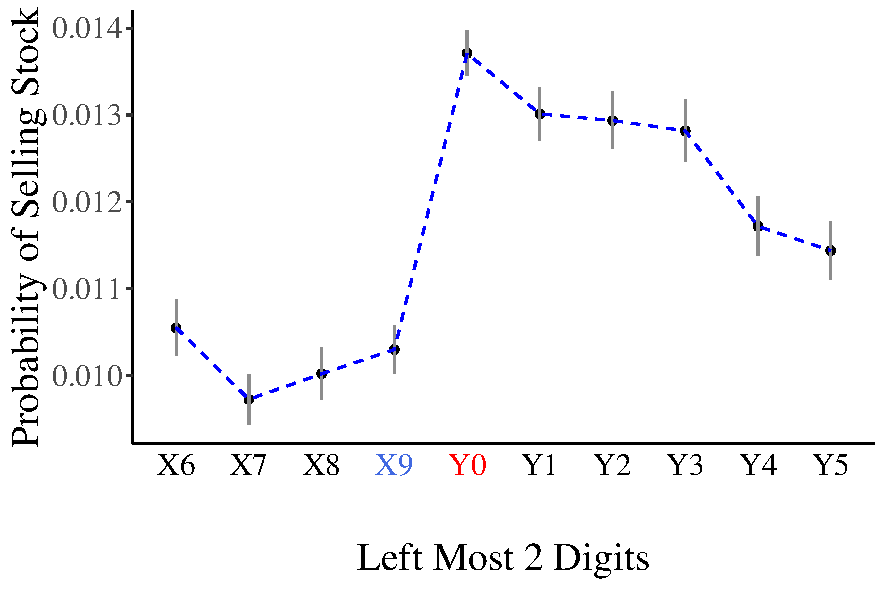
\includegraphics[width=0.45\textwidth]{figures/Left2increase_probCI_year.pdf}
		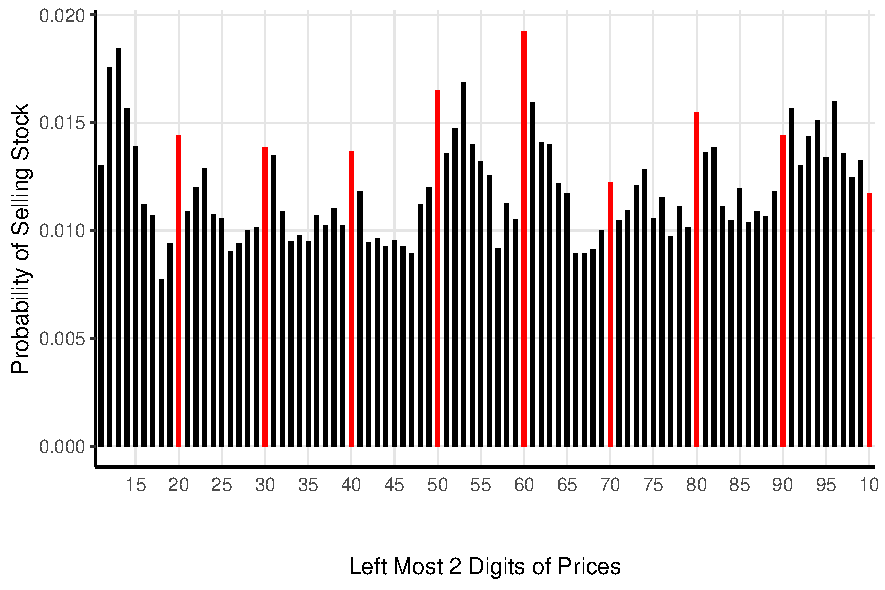
\includegraphics[width=0.45\textwidth]{figures/2left_increase_year.pdf}	
	}
	\subfigure[Price Decreasing]{
		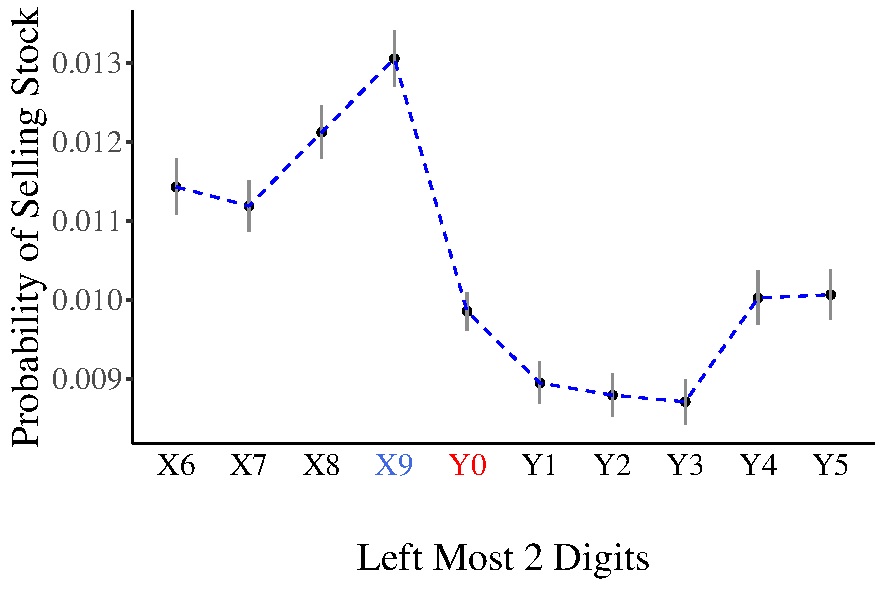
\includegraphics[width=0.45\textwidth]{figures/Left2decrease_probCI_year.pdf}
		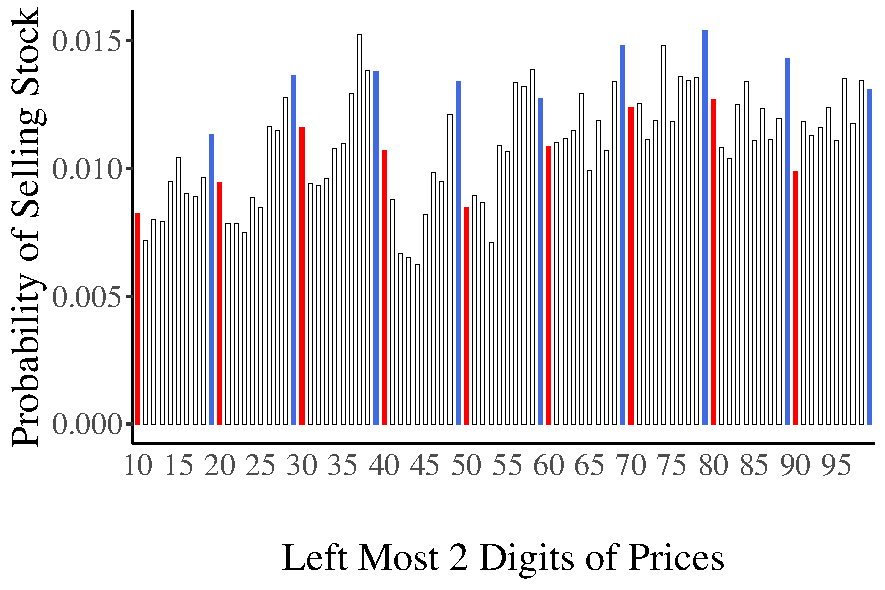
\includegraphics[width=0.45\textwidth]{figures/2left_decrease_year.pdf}	
	}
	\fignote{£$Y$ in the X-axes is equivalent to £$X+1$ (e.g., £X9 could include £0.19, £1.9, £19, etc., while £Y0 could include £0.20, £2.0, £20, etc.).}
\end{figure}

\clearpage
\textcolor{blue}{EQ: Robustness 3: Random sells (using the same samples of our main analysis, quarterly sample and login days)}

\begin{figure}[hbt!]
	\caption{Sample Selection and Simulation Exercise}%
	\label{fig:sample_selection_test}%
	\centering%	
	\bigskip
	\subfigure[Price Increasing Sample]{
		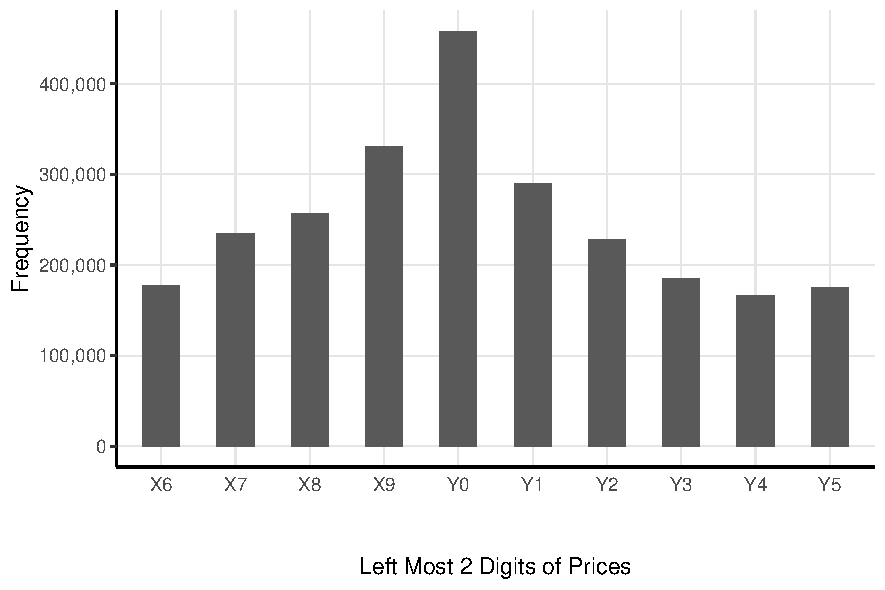
\includegraphics[width=0.45\textwidth]{figures/left2_second_increase_count_quarter.pdf}
		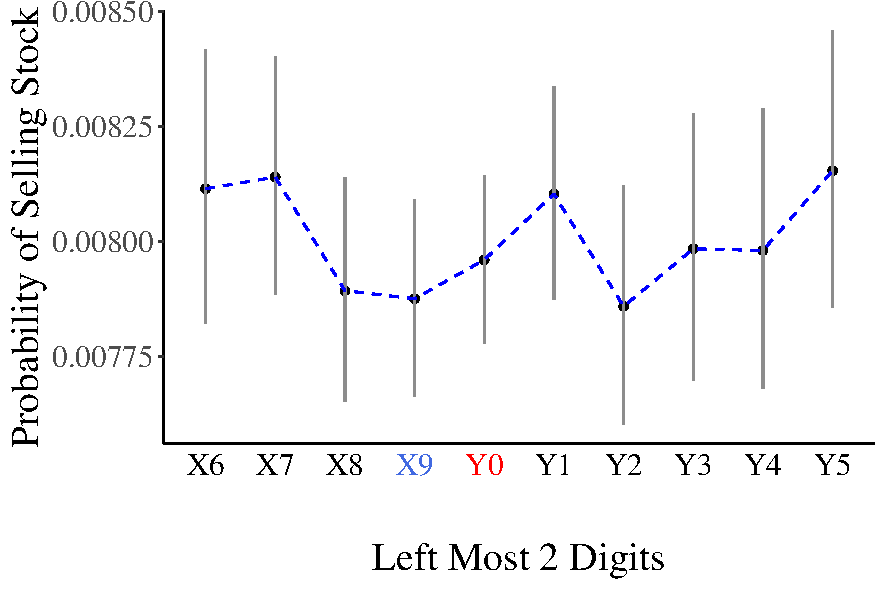
\includegraphics[width=0.45\textwidth]{figures/Left2increase_probCI_quarter_random_sell.pdf}
	}
	\subfigure[Price Decreasing Sample]{
	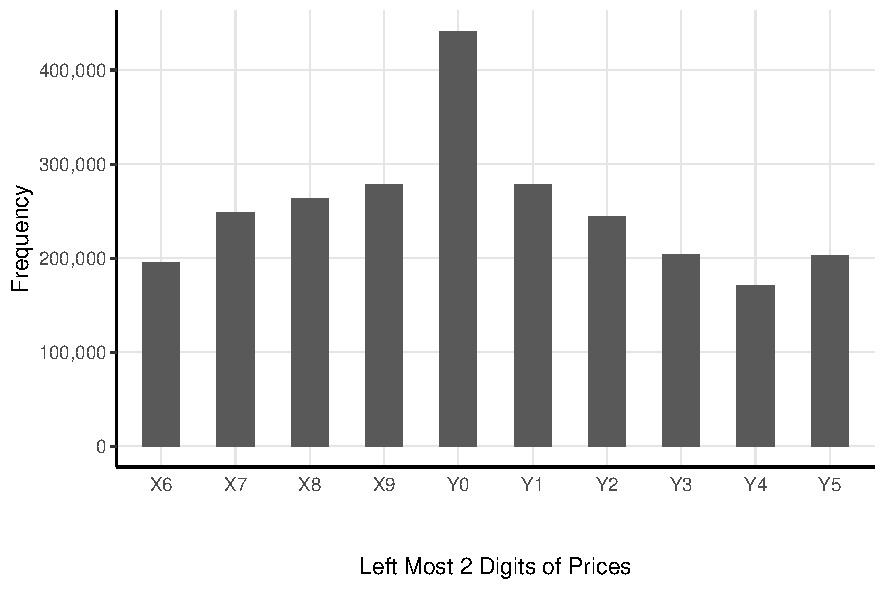
\includegraphics[width=0.45\textwidth]{figures/left2_second_decrease_count_quarter.pdf}
	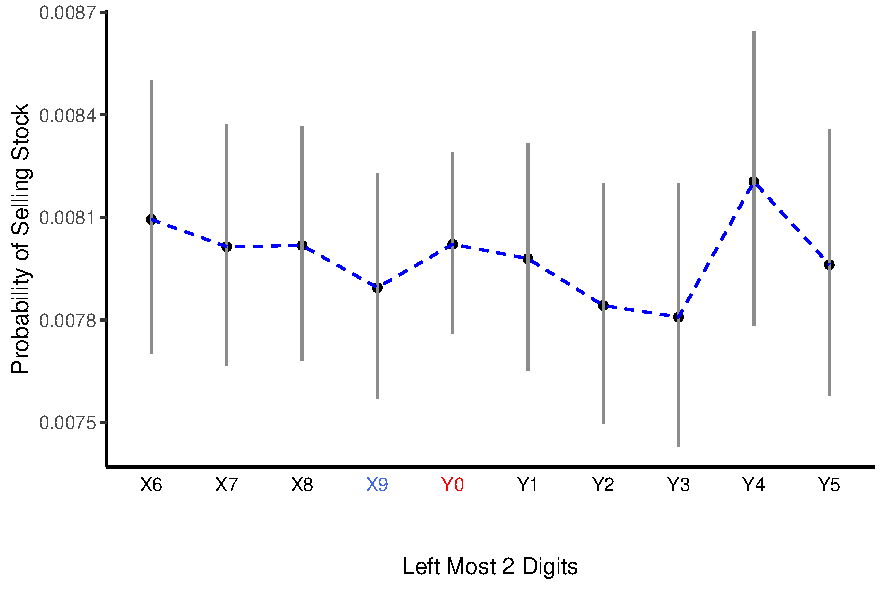
\includegraphics[width=0.45\textwidth]{figures/Left2decrease_probCI_quarter_random_sell.pdf}
}
\end{figure}

\clearpage
\textcolor{blue}{EQ: Robustness 4 [part 1]: Same patterns in sell days (quarterly sample and sell days)}


\begin{figure}[hbt!]
	\caption{Leftmost Stock Price Digit and Probability of Sale, Sell Days}%
	\label{fig:left_digit_sell}%
	\centering%	
	\bigskip
	\subfigure[Price Increasing]{
		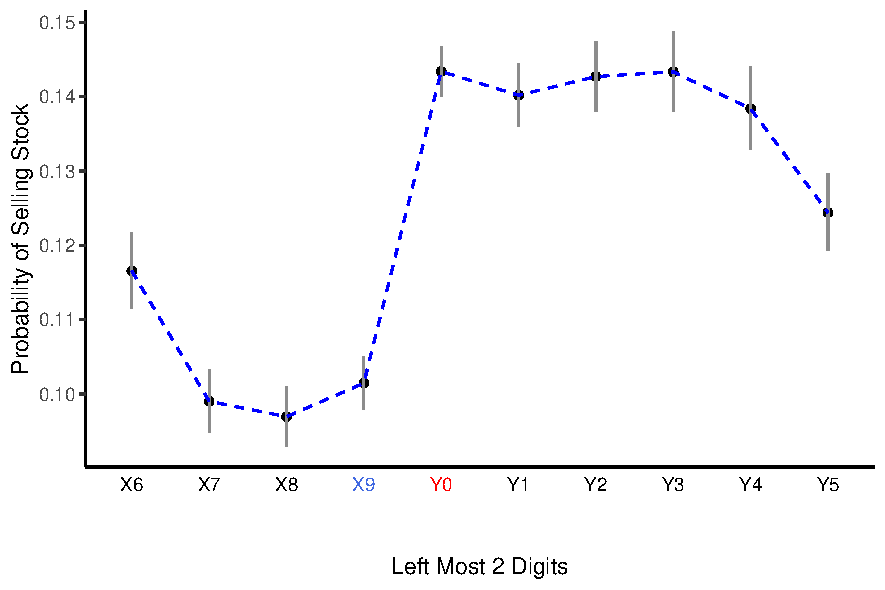
\includegraphics[width=0.45\textwidth]{figures/Left2increase_probCI_quarter_sell.pdf}
		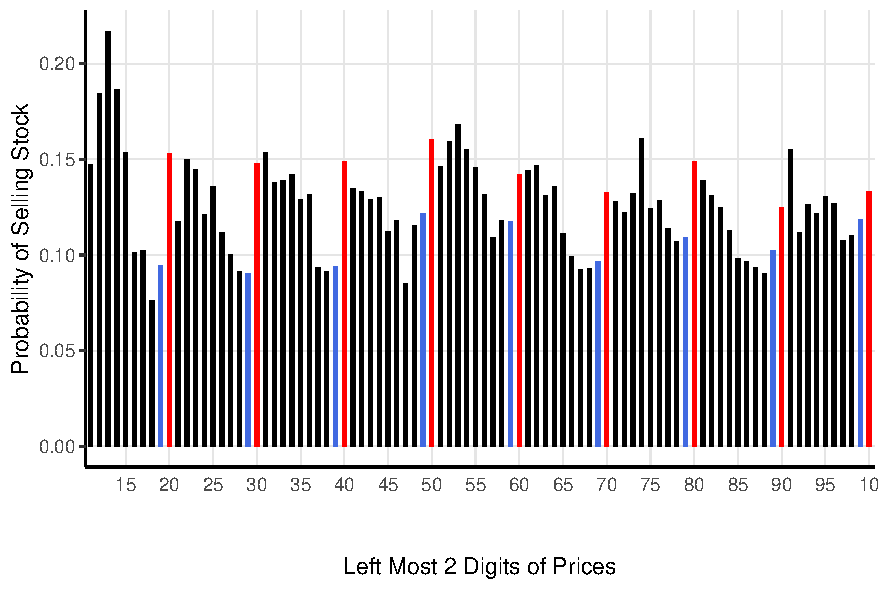
\includegraphics[width=0.45\textwidth]{figures/2left_increase_quarter_sell.pdf}	
	}
	\subfigure[Price Decreasing]{
		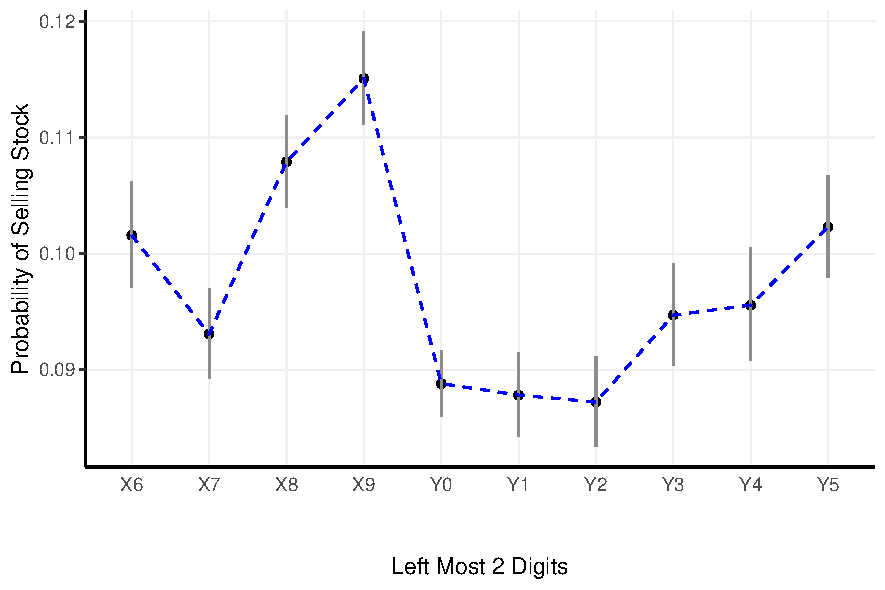
\includegraphics[width=0.45\textwidth]{figures/Left2decrease_probCI_quarter_sell.pdf}
		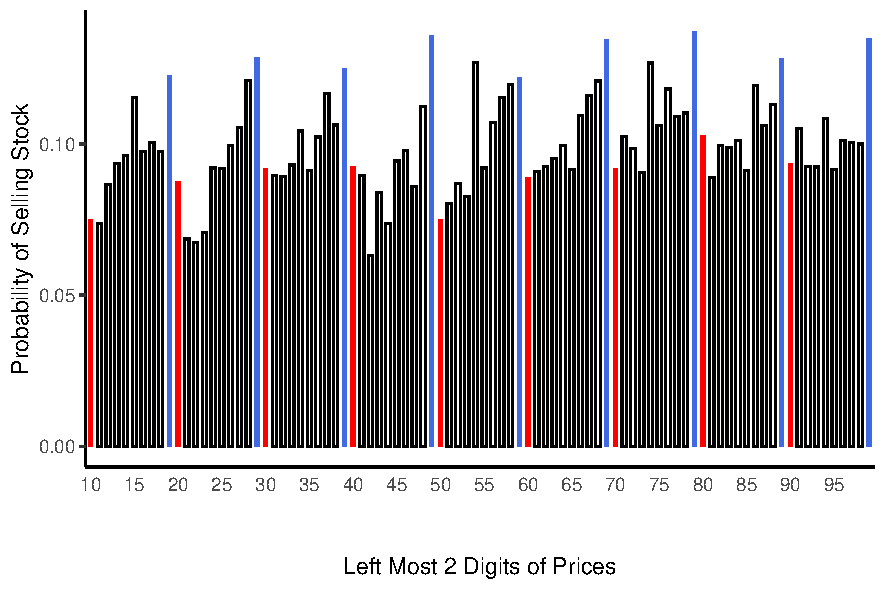
\includegraphics[width=0.45\textwidth]{figures/2left_decrease_quarter_sell.pdf}	
	}
	\fignote{£$Y$ in the X-axes is equivalent to £$X+1$ (e.g., £X9 could include £0.19, £1.9, £19, etc., while £Y0 could include £0.20, £2.0, £20, etc.).}
\end{figure}

\clearpage
\textcolor{blue}{EQ: Robustness 4 [part 2]: Same patterns in sell days, sub-samples of equal bin size for our main sample (quarterly sample and sell days)}

\begin{figure}[hbt!]
	\caption{Leftmost Stock Price Digit and Probability of Sale, Sell Days \\ Prices Increasing Sample by Price Range}%
	\label{fig:left_digit_sell_increase}%
	\centering%	
	\bigskip
	\subfigure[Price = \pounds0.11 to \pounds1.01]{
		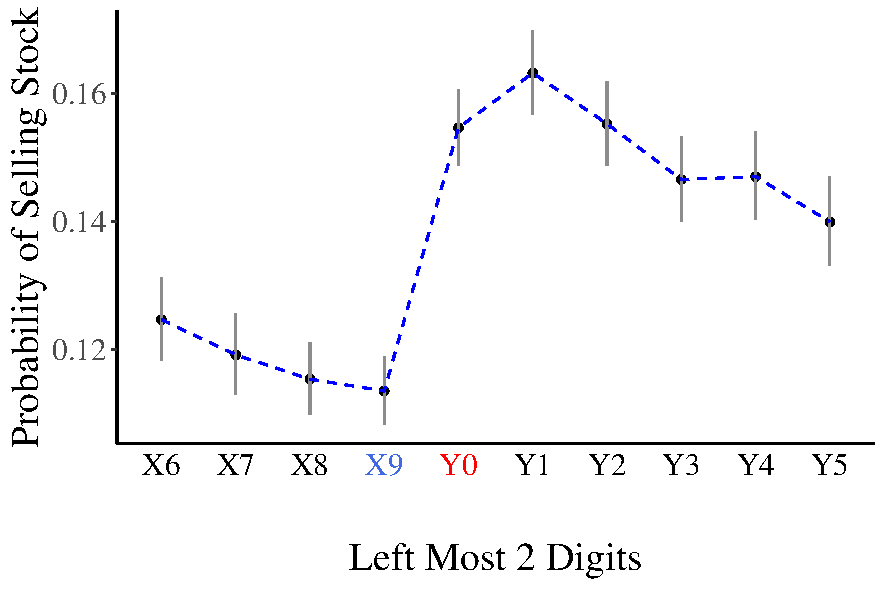
\includegraphics[width=0.45\textwidth]{figures/Left2increases_1pbin_CI_quarter_sell.pdf}
		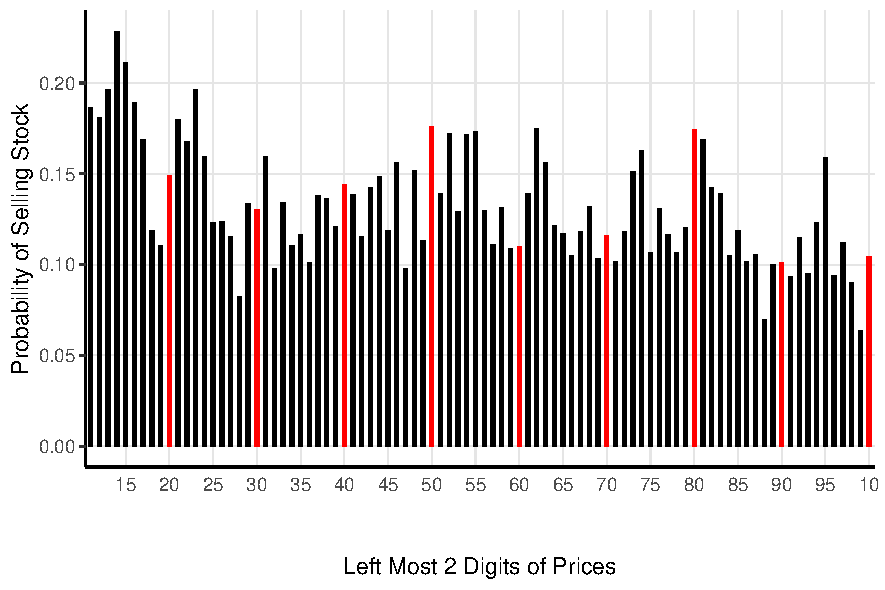
\includegraphics[width=0.45\textwidth]{figures/2left_increase_bin1p_quarter_sell.pdf}
	}
	\subfigure[Price = \pounds1.01 to \pounds10.1]{
		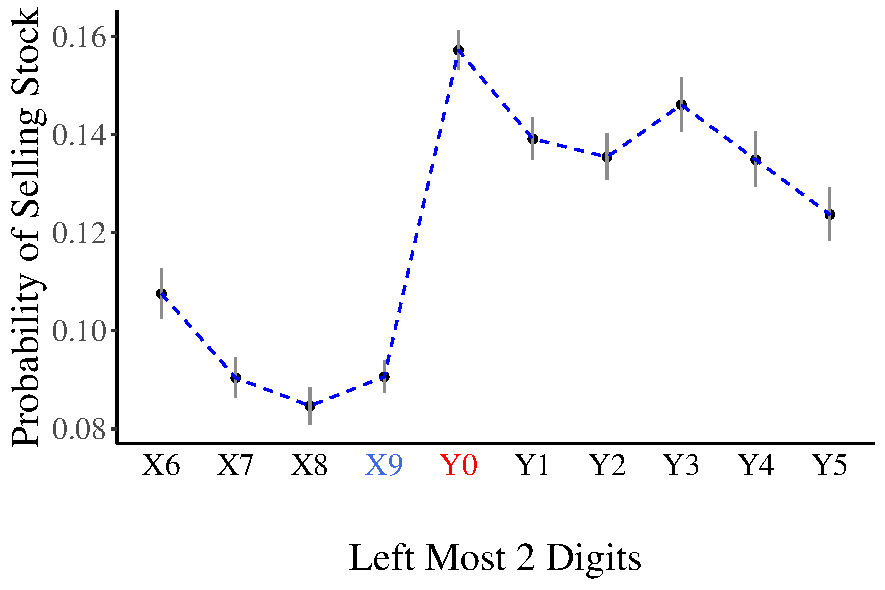
\includegraphics[width=0.45\textwidth]{figures/Left2increases_10pbin_CI_quarter_sell.pdf}
		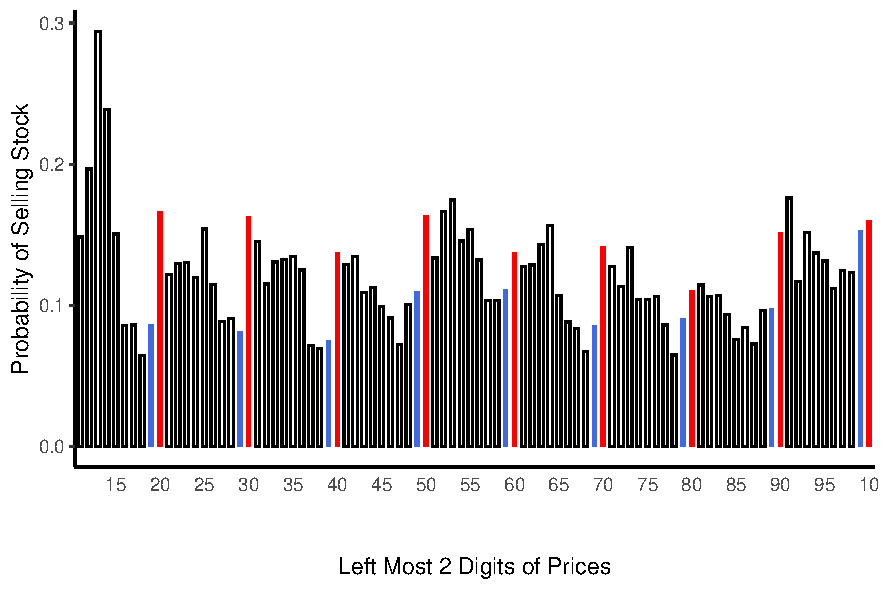
\includegraphics[width=0.45\textwidth]{figures/2left_increase_bin10p_quarter_sell.pdf}
	}
	\subfigure[Price = \pounds11 to \pounds101]{
		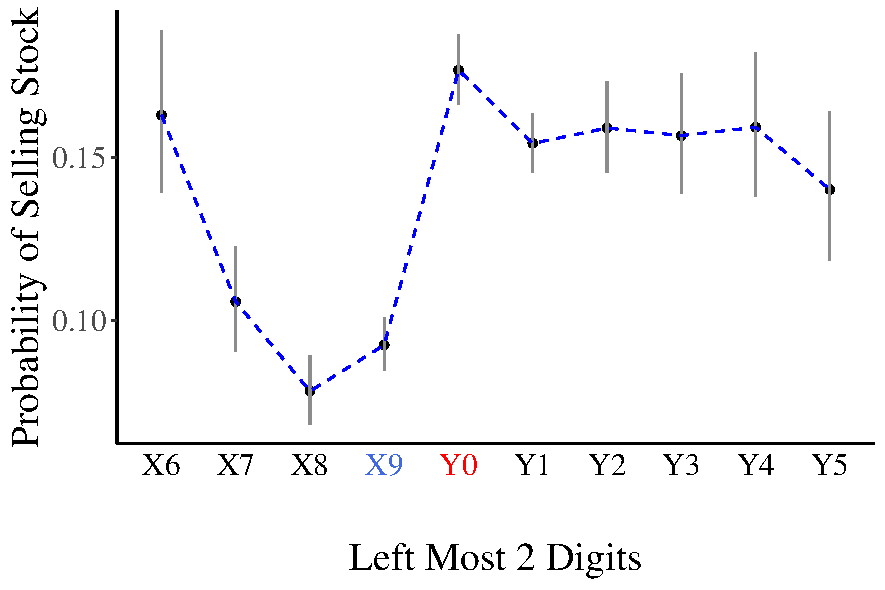
\includegraphics[width=0.45\textwidth]{figures/Left2increases_1poundbin_CI_quarter_sell.pdf}
		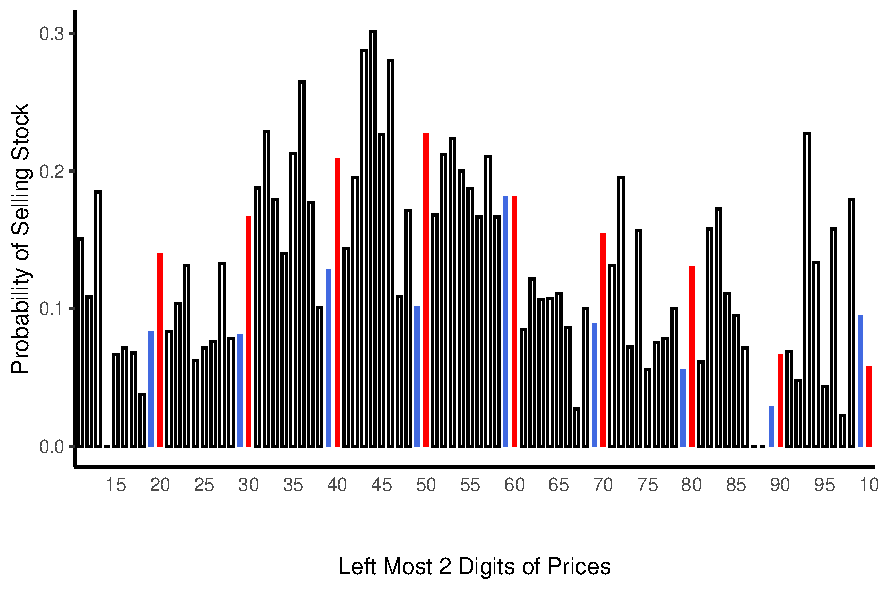
\includegraphics[width=0.45\textwidth]{figures/2left_increase_bin1pound_quarter_sell.pdf}
	}
	\fignote{£$Y$ in the X-axes is equivalent to £$X+1$ (e.g., £X9 could include £0.19, £1.9, £19, etc., while £Y0 could include £0.20, £2.0, £20, etc.). Panels A, B and C show equal size bins of 1p, 10p and £1, respectively. }
\end{figure}

\begin{figure}[hbt!]
	\caption{Leftmost Stock Price Digit and Probability of Sale, Sell Days \\ Prices Decreasing Sample by Price Range}%
	\label{fig:left_digit_sell_decrease}%
	\centering%	
	\bigskip
	\subfigure[Price = \pounds0.10 to \pounds1.00]{
		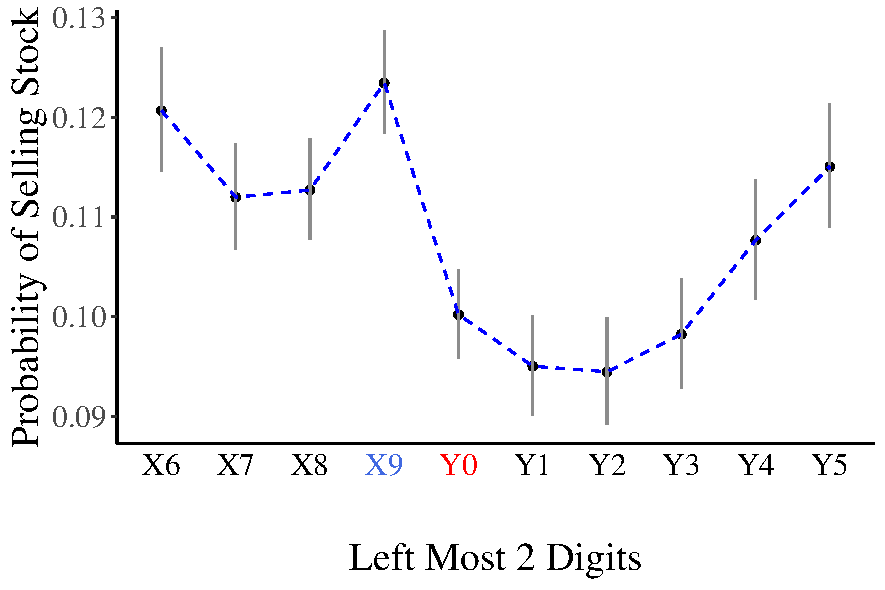
\includegraphics[width=0.45\textwidth]{figures/Left2decreases_1pbin_CI_quarter_sell.pdf}
		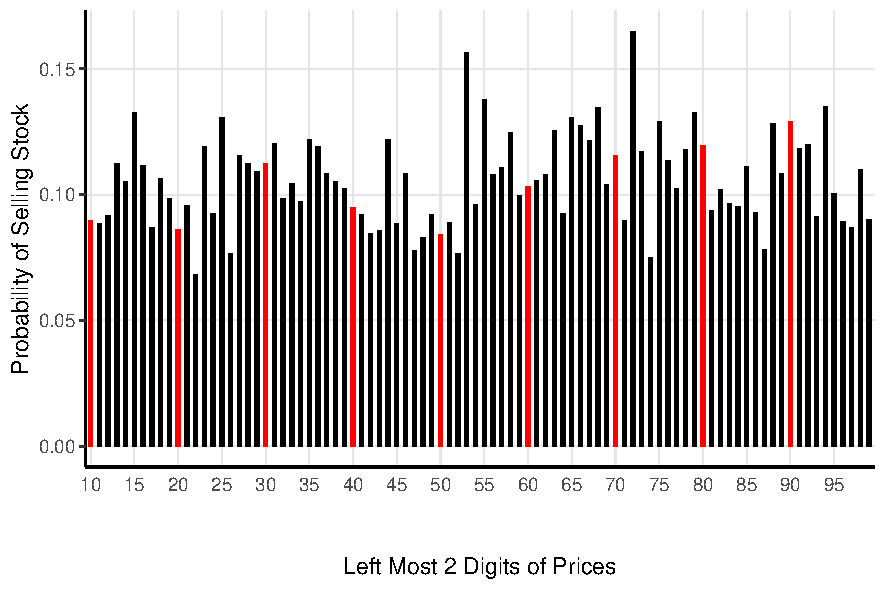
\includegraphics[width=0.45\textwidth]{figures/2left_decrease_bin1p_quarter_sell.pdf}
	}
	\subfigure[Price = \pounds1.00 to \pounds10.0]{
		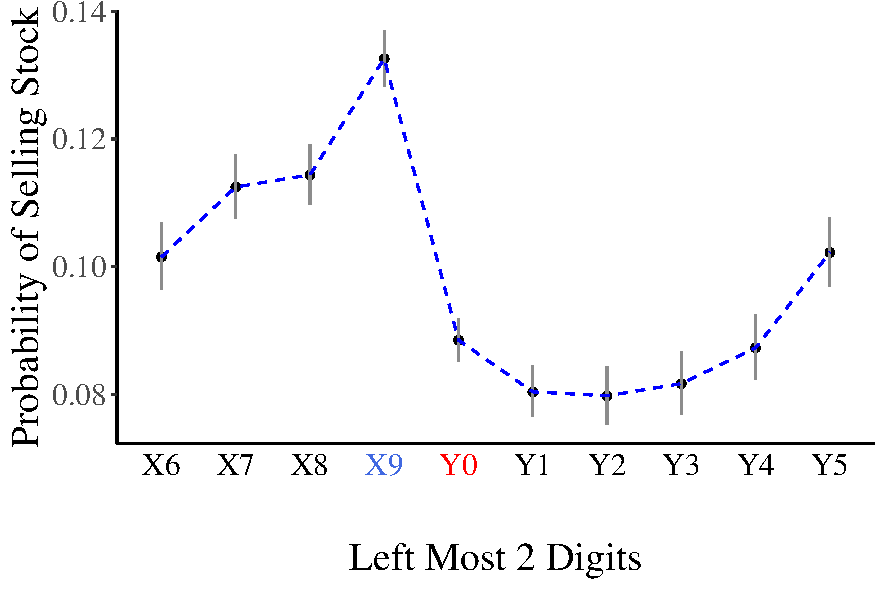
\includegraphics[width=0.45\textwidth]{figures/Left2decreases_10pbin_CI_quarter_sell.pdf}
		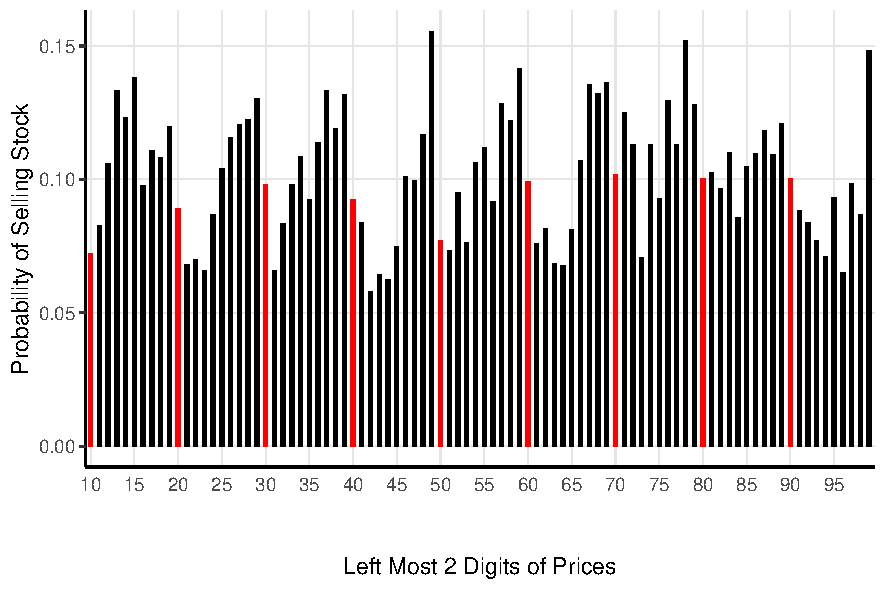
\includegraphics[width=0.45\textwidth]{figures/2left_decrease_bin10p_quarter_sell.pdf}
	}
	\subfigure[Price = \pounds10 to \pounds100]{
		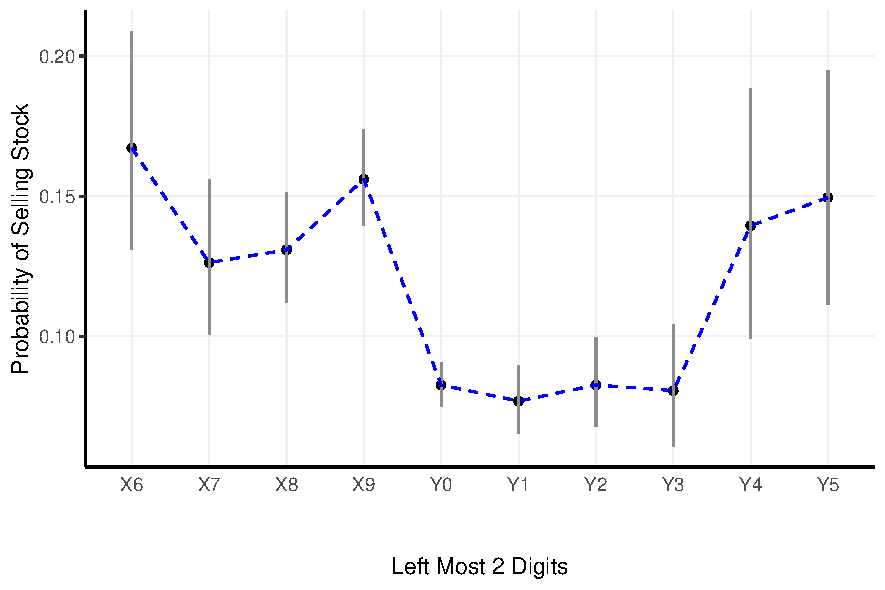
\includegraphics[width=0.45\textwidth]{figures/Left2decreases_1poundbin_CI_quarter_sell.pdf}
		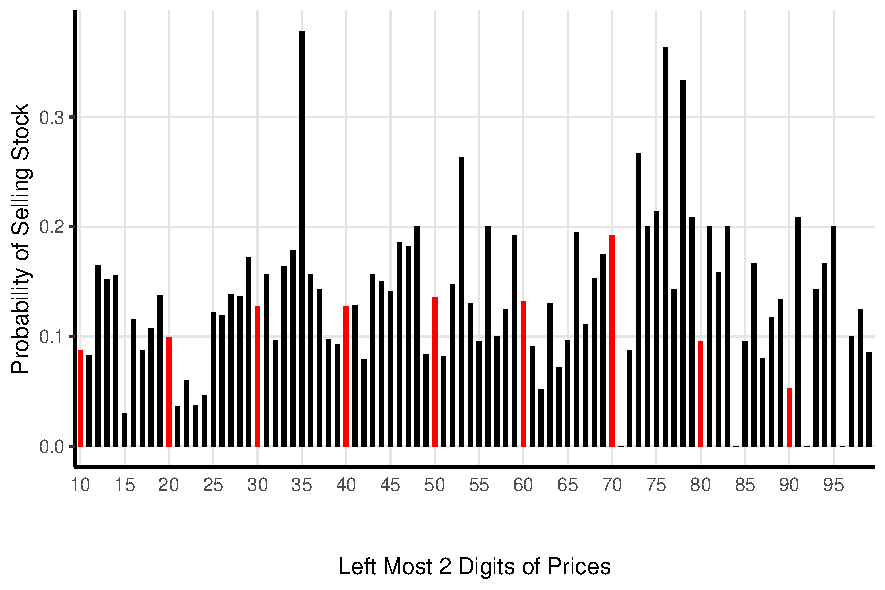
\includegraphics[width=0.45\textwidth]{figures/2left_decrease_bin1pound_quarter_sell.pdf}
	}
	\fignote{£$Y$ in the X-axes is equivalent to £$X+1$ (e.g., £X9 could include £0.19, £1.9, £19, etc., while £Y0 could include £0.20, £2.0, £20, etc.). Panels A, B and C show equal size bins of 1p, 10p and £1, respectively. }
\end{figure}



\begin{figure}[hbt!]
	\caption{Probability of Topping-up \textcolor{blue}{[EQ: I remember we talked with George about doing the topping up analysis. Perhaps we could just tell him that the analysis did not work and drop this plot? What do you think? Just in case, I am leaving the plots here for now. These plots were done using new accounts. ]}}%
	\label{fig:topup}%
	\centering%	
	\bigskip
	\subfigure[Price Increasing Sample]{
		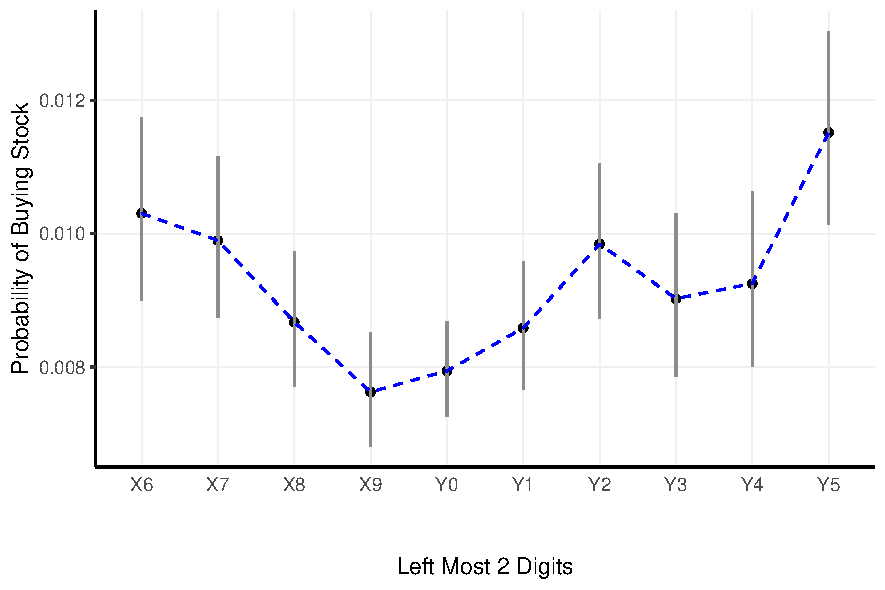
\includegraphics[width=0.70\textwidth]{figures/Left2increase_probCI_top_up.pdf}
	}
	\subfigure[Price Decreasing Sample]{

	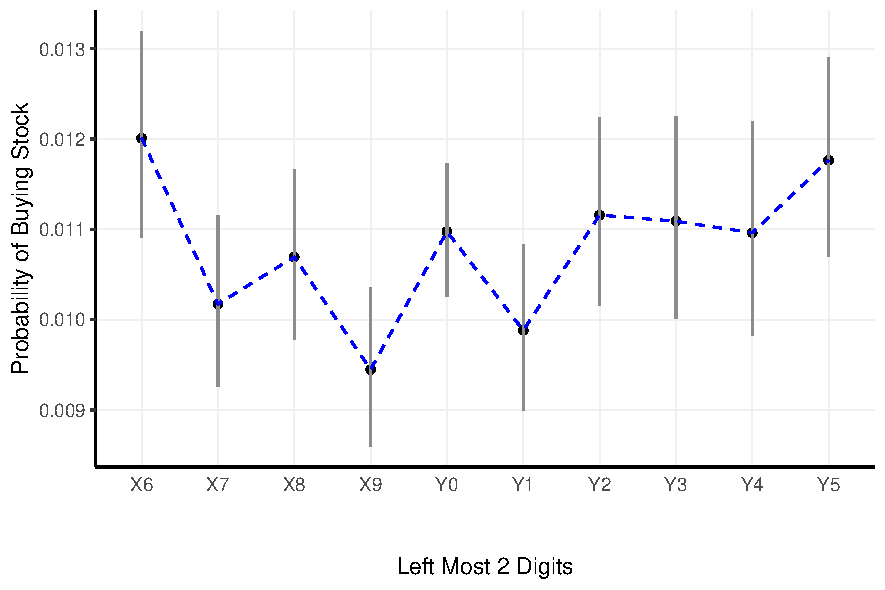
\includegraphics[width=0.70\textwidth]{figures/Left2decrease_probCI_top_up.pdf}
}
	\fignote{Figure shows the probability of topping up (increasing position in an stock) under the same sample selection. 	£$Y$ in the X-axes is equivalent to £$X+1$ (e.g., £X9 could include £0.19, £1.9, £19, etc., while £Y0 could include £0.20, £2.0, £20, etc., ).}
\end{figure}


